\chapter{Evaluation}\label{s:evaluation}

\section{Design of experiment}
The research is based on a theory stating privacy breaches of citizens are a growing issue and technologies could be applied more broadly to mitigate it. In the design phase of the experiment it seemed to be a clear scope, focusing on parts like UIN to be a problem and techniques of tokenization and pseudoymization to be a possible solution. During the research it became clear more research and refinement was needed on a solvable part of a bigger problem. Also, only taking two techniques in account as a possible solution seemed too narrow in hindsight.

Therefore, theory of the problem was gained through literature study and a practical understanding was gathered via semi-structured interviews.

\section{Methodology}
Research method is an inductive exploratory approach, based on the theory technologies could support privacy preservation of citizens. Also, research is from an interpretive kind, because understanding the possible problems is part of it.

Experts where consulted on bringing focus to the research problem and scope. These consulted experts referred to available literature and therefore these conversations where not recorded and transcribed. 
Semi-structured interviews where used for the same reason, but are used to get a more detailed view. The interviews are transcribed and information is extracted by using the coding method.  Williams and Moser \cite{Williams2019TheAO} claim: "Regardless of the research approach, the methodology employed for data collection and
organization must be clear and repeatable, leading to and enabling data analysis..... A key data organizing structure in qualitative research is coding." This is why coding method has been used. 

\graphicspath{ {./images/} }
\begin{figure}
\centering
\label{fig:WM2019}
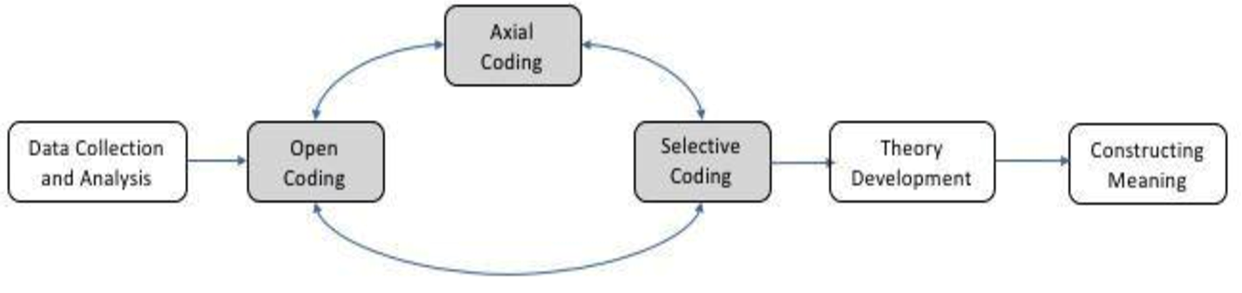
\includegraphics[width=14cm]{Williams and Moser.png}\\
\caption{Non-Linear Process. Williams and Moser \cite{Williams2019TheAO} Figure 3}
\end{figure}

Firstly transcribing the interviews is part of the "Data collection and Analysis" phase. "Open coding" has been done by marking possible interesting parts, based on the themes of Business Goals and Concerns. The step of "Axial coding" results in refinement to Quality attributes of ISO-25010. Defining Quality Attributes considered Architectural Significant refinements are defined in the last part of "Selective Coding". The "Theory Development" and "Constructing Meaning" phase are result in Attribute refinemets and Quality Attribute scenarios. Section \ref{s:overview} contains the Utility tree to depict the cohesion between these steps. In this way coding has been applied on methodology described in Software Architecture in Practice of Bass\etal \cite{Bass2015SoftwareAI}.

Biases will be discussed in the section 'Threats to validity'

\section{Obtained results}
Themes in the form of Business Goals and Concerns are included in Appendix \ref{Appendix B} and Appendix \ref{Appendix C}. The results of translating them to Quality Attributes and Attribute Refinements in Figure \ref{fig:ASR1} combining them with the Business Goals and Concerns in Table \ref{ASR_BG_C}.



%\todo{
%Discuss the design of your experiments, the results you obtained, and how they
%help in evaluating the claims you made in the introduction. You may also use the
%evaluation results in this section to justify your design choices or assess the
%contributions of different aspects  of your design towards the overall goals.
%}

